\newpage
\section{Problem I \ \ Superdog的菌毯肿瘤}
{ \limitfont{}
Input file: Standard Input \par
Output file: Standard Output \par
Time limit: 1000ms \par
Memory limit: 512MB \par
}
\subsection*{题目描述}
作为一个星际争霸2的虫族玩家,Superdog非常擅长拓张自己的领土:菌毯。众所周知,虫族的菌毯是靠菌毯肿瘤扩大覆盖范围的,如果菌毯肿瘤被敌人消灭,菌毯就会慢慢消失。并且,Superdog发现,任意两个菌毯肿瘤的连线所构成的开线段都在菌毯内部。简而言之,菌毯的范围是所有菌毯肿瘤构成的凸面。

Superdog突发奇想,他希望在已有的菌毯上建造新的建筑。但是他发现,菌毯肿瘤的存在会阻碍建筑的建造,所以他希望能在菌毯找到最大的一块菌毯空地,且这个空地也是一个凸面。

在下图中,菌毯组成的凸面为虚线标注的部分,用实线标注的部分是Superdog找到最大的菌毯空地。
\begin{figure}[H]
    \centering
    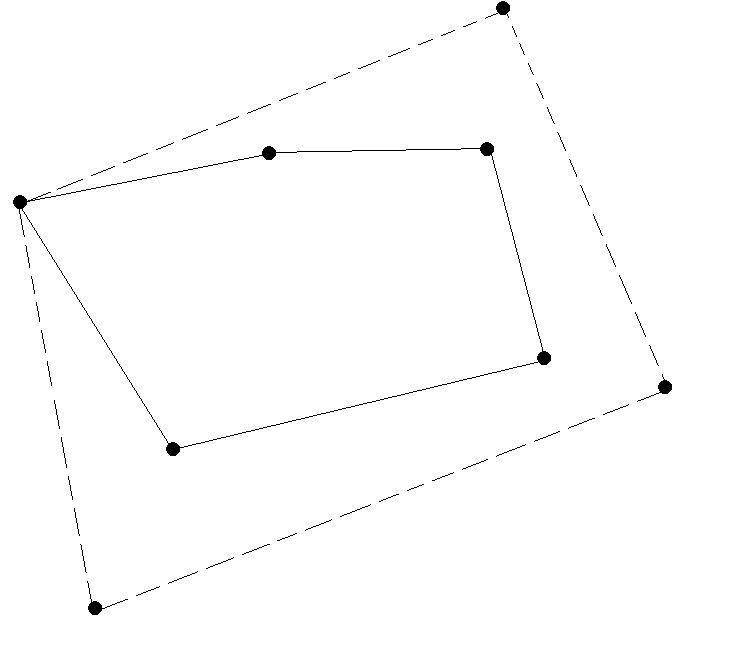
\includegraphics[scale=0.6]{./src/k.png}
\end{figure}
\subsection*{输入描述}

第一行一个整数$T$,代表有$T$组输入。

对于每组输入,第一行有一个整数$n$,代表有$n$个菌毯肿瘤,保证没有重复的菌毯肿瘤。

接下来n行,每行两个整数$x_i,y_i$代表第i个菌毯肿瘤的坐标。

\subsection*{输出描述}

一个浮点数,代表最大菌毯空地的面积,如果和正确答案的误差小于$10^{-3}$,Superdog则认为答案正确。

\subsection*{测试样例}

\begin{table}[H]
\begin{tabularx}{\textwidth}{|X|X|}
    \hline
    \textbf{Standard Input} & \textbf{Standard Output} \\ 
    \hline 
    \tablecell{
        2 \\
        5 \\
        1 1 \\
        2 2 \\
        3 3 \\
        0 0 \\
        5 1 \\
        6 \\
        0 0 \\
        0 1 \\
        0 2 \\
        1 1 \\
        1 2 \\
        2 1 \\
    } & 
    \tablecell{
        6.0000 \\
        1.5000 \\
        \\ \\ \\ \\ \\ \\ \\ \\ \\ \\ \\ \\
    } \\
    \hline
\end{tabularx}
\end{table}
\subsection*{数据规模}
$1< T \leq 100$

$2<n \leq 100$

$0 \leq x,y \leq 1000$